\section{Overfit ve Underfit}
Overfitting, bir modelin eğitim verilerine aşırı derecede uyum sağlaması ve genelleme yapma yeteneğini kaybetmesi durumudur. Overfitting durumunda, model eğitim verilerine çok iyi uyum sağlar, ancak yeni, görünmemiş verilere karşı uyumsuz olur. Model eğitim sürecinde, model karmaşıklığı arttıkça, overfitting riski artar.  Overfitting, modelin gürültüye veya eğitim verilerindeki örneklem hatalarına aşırı derecede tepki göstermesiyle ortaya çıkabilir.

Underfitting, bir modelin eğitim verilerine yeterince uyum sağlayamaması ve veri setindeki örüntüleri yeterince yakalayamaması durumudur. Underfitting durumunda, model hem eğitim verilerine hem de yeni verilere kötü bir şekilde uyum sağlar, yani modelin performansı düşüktür.  Model karmaşıklığı çok düşük olduğunda veya modelin eğitim süreci yeterince uzun olmadığında underfitting oluşabilir.  Underfitting, modelin gereğinden fazla basit olduğu durumlarda veya yeterince eğitim verisi olmadığında ortaya çıkabilir.

\begin{figure}[h]
    \centering
    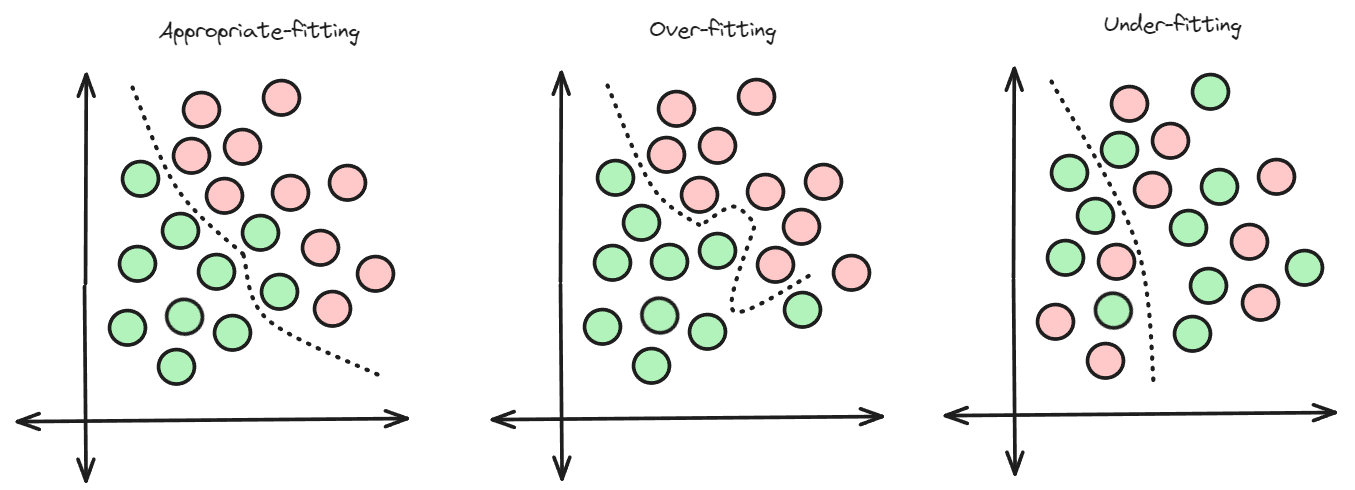
\includegraphics[width=1\textwidth]{images/overfit_vs_underfit.png}
    \caption{Overfit ve Underfit}
    \label{fig:enter-label}
\end{figure}

\newpage